\documentclass{standalone}
\usepackage[utf8]{inputenc}
\usepackage[svgnames]{xcolor}
\usepackage{tikz}
\usetikzlibrary{fit,shapes,positioning}


\begin{document}
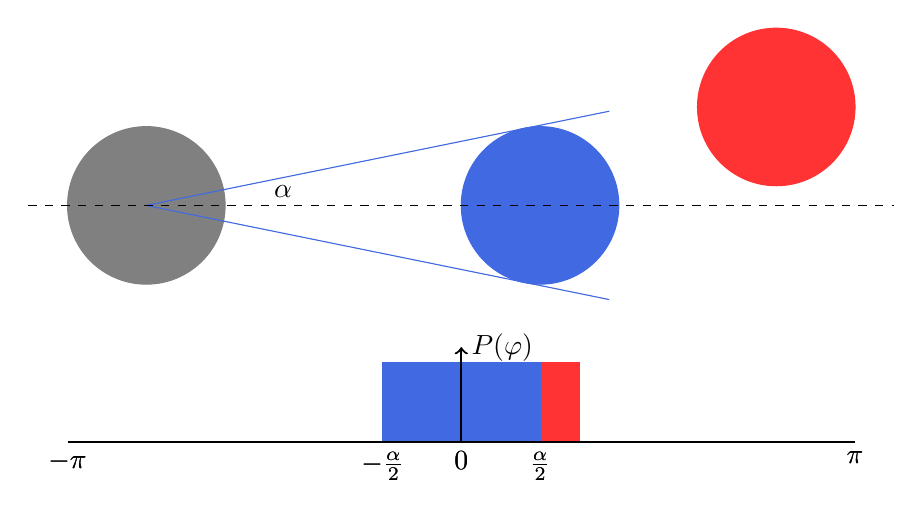
\begin{tikzpicture}[
        graph/.style={fill=black, draw opacity=0, fill opacity=0.5},
        friend/.style={color=RoyalBlue, fill=RoyalBlue},
        enemy/.style={color=red!80!white, fill=red!80!white}
    ]
    
    \filldraw[gray]    (0,0) circle (1cm) coordinate (a) ;
    \filldraw[friend]  ([xshift=5cm]a) circle (1cm) coordinate (b) ;
    \filldraw[enemy]   ([xshift=8cm,yshift=1.25cm]a) circle (1cm) coordinate (c) ;
    \draw[friend] (a) -- (11.5:6cm)  ;
    \draw[friend] (a) -- (-11.5:6cm) ;

    \draw[dashed] ([xshift=-1.5cm]a) -- ([xshift=1.5cm]a -| c) ;
    \node[right=1.5cm of a, yshift=0.5em] {$\alpha$} ;


    \coordinate (x0) at ([xshift=-1cm, yshift=-3cm]a) ;
    \coordinate (x1) at ([xshift=1cm]x0 -| c) ;

    % calc coordinates
    \draw[thick] (x0) to
        node[pos=0,below]{$-\pi$}
        node[pos=0.4,below]{$-\frac{\alpha}{2}$} coordinate[pos=0.4] (alpha0)
        node[pos=0.5,below]{$0$} coordinate[pos=0.5] (y0)
        node[pos=0.6,below]{$\frac{\alpha}{2}$} coordinate[pos=0.6] (alpha1)
        coordinate[pos=0.65] (beta1)
        node[pos=1,below]{$\pi$} (x1);

    \draw[enemy] (alpha1) rectangle ([yshift=1cm]beta1)  ;
    \draw[friend] (alpha0) rectangle ([yshift=1cm]alpha1)  ;

    
    \draw[thick, ->] (y0) -- ([yshift=1.2cm]y0) node[right]{$P(\varphi)$} ;
    \draw[thick] (x0) to
        node[pos=0,below]{$-\pi$}
        node[pos=0.4,below]{$-\frac{\alpha}{2}$} coordinate[pos=0.4] (alpha0)
        node[pos=0.5,below]{$0$} coordinate[pos=0.5] (y0)
        node[pos=0.6,below]{$\frac{\alpha}{2}$} coordinate[pos=0.6] (alpha1)
        node[pos=1,below]{$\pi$} (x1);

    
\end{tikzpicture}
\end{document}